\section{Brownian boundaries and Williams' structure}\label{ch:boundaries}

Under RH with simple zeros, Kent's theorem makes the clock variable $T$ the hitting time of a level by a diffusion, but it describes that diffusion only through its spectrum, the set $\{\gamma^2\}$ that is to be found (Section~\ref{sec:ch18:kent}). We look instead for a representation by Brownian motion itself. Unconditionally, $T$ is not a Brownian first passage time to an independent random level for any constant drift (Section~\ref{sec:ch19:nogo}). Across a curved boundary it is one: such a boundary exists by a theorem of Ekstr\"om and Janson, and we compute it (Section~\ref{sec:hitting}). Williams' representation of the P\'olya kernel through Bessel hitting times explains the tilted contour of Section~\ref{sec:newcomp}, but it transfers no positivity to the clock (Section~\ref{sec:ch19:williams}).

\subsection{The clock is not a first passage time to a random level}\label{sec:ch19:nogo}

The first passage time of Brownian motion with drift $c\ge0$ to a level $a>0$ has the inverse Gaussian law, with transform $\exp\{a(c-\sqrt{c^2+2u})\}$. Mixing over an independent random level with law $F$ gives the transforms $\int\exp\{a(c-\sqrt{c^2+2u})\}F(da)$, a class of first passage laws.

\begin{proposition}\label{prop:nogo}
For no drift $c\ge0$ and no probability law $F$ on $(0,\infty)$ is the clock variable $T$ equal in law to the first passage time of Brownian motion with drift $c$ to an independent level $A\sim F$.
\end{proposition}

\begin{proof}
On the parabola $u=\tfrac12(-q^2+2icq)$, $q\in\mathbb R$, we have $c^2+2u=(c+iq)^2$, so $\re\sqrt{c^2+2u}=c$ and every mixture transform has modulus at most one there. Suppose that $T$ had such a law, so that the clock transform $1/G(u)=\E e^{-uT}$ and the mixture transform agree for $u\ge0$. The mixture transform is analytic and bounded by one on the region $D=\{u:\re\sqrt{c^2+2u}>c\}$, and continuous up to its boundary, which is the parabola. The region $D$ is the image of the half plane $\re v>c$ under $v\mapsto(v^2-c^2)/2$, so it is connected, and it contains the right half plane. By the identity theorem $1/G$ coincides with the mixture transform on $D$, so it has no pole in $D$ and is bounded by one there, and by continuity $|1/G|\le1$ on the parabola away from the zeros of $\xi(\tfrac12+\sqrt u)$. For the clock, however, $\sqrt u=(c+iq)/\sqrt2+O(1/q)$ as $q\to\infty$ (for $c=0$ the parabola is the negative axis, approached from above, and $\sqrt u=i|q|/\sqrt2$), so $|\xi(\tfrac12+\sqrt u)|$ decays like $\exp(-\pi|q|/(4\sqrt2))$ times a power, by Stirling's formula and the polynomial growth of $\zeta$ in vertical strips. Hence $|\xi(\tfrac12)/\xi(\tfrac12+\sqrt u)|$ grows exponentially along the parabola, and the transforms cannot agree.
\end{proof}

The proof covers the nonincreasing lines $a-ct$, $c\ge0$; an increasing line, with $c<0$, gives a passage time that is infinite with probability $1-\E e^{2cA}>0$, which the clock is not. Expanding $G(u)=1+m_1u+m_2u^2+\cdots$ with $m_1=\E T$ and $m_1^2-2m_2=\mathrm{Var}\,T$ gives $|G(u)|^2=1-q^2(m_1-c^2\,\mathrm{Var}\,T)+O(q^3)$ on the parabola, so the clock transform already exceeds one at small $q$ whenever
\[
c<c_*=\sqrt{\E T/\mathrm{Var}\,T}=\sqrt{0.0231050/3.71726\times10^{-5}}=24.93 .
\]


\subsection{A curved Brownian boundary for the clock}\label{sec:hitting}

Finding a boundary whose first passage time has a prescribed law is the inverse first passage problem \cite[Theorem 1]{CCCS11}. By the theorems of Ekstr\"om and Janson \cite[Theorems 2.3, 8.2 and 9.2]{EkstromJanson16}, stated in full in Section~\ref{bp:sec:rs1}, the problem has a solution for the clock, which we call the exact boundary. Since the density of the clock is continuous and positive on $(0,\infty)$ (Exercise~\ref{ex:ch19:density}), the same theorems make the exact boundary continuous on $(0,\infty)$ and the unique continuous solution $b$ with $\liminf_{t\downarrow0}b(t)\ge0$ of the Volterra integral equation \eqref{eq:ch19:volterra} of the first passage density. We call the solution of the discretised Volterra equation the Volterra boundary.

\subsubsection{The Roberts Shortland tangent boundary}\label{sec:ch19:tangent}

Roberts and Shortland \cite{RS95} approximate the hazard of a Brownian first passage across a smooth boundary $b$ by the hazard of the tangent line at the current time, for which the Bachelier L\'evy formula is exact:
\begin{gather*}
h_{\rm tan}(t)=\frac{\alpha(2\pi t^3)^{-1/2}\exp\{-(\alpha+\beta t)^2/2t\}}{\mathcal N\big((\alpha+\beta t)/\sqrt t\big)-e^{-2\alpha\beta}\mathcal N\big((\beta t-\alpha)/\sqrt t\big)},\\
\beta=b'(t),\ \alpha=b(t)-tb'(t),
\end{gather*}
where $\mathcal N$ is the standard normal distribution function; we write $\overline{\mathcal N}=1-\mathcal N$ for its tail. We use the formula in reverse. Setting $h_{\rm tan}(t)=h(t)$, the computed hazard of the clock, defines an ordinary differential equation for $b$, which we integrate by the fourth order Runge Kutta method with step $10^{-4}$ from $t_0=0.011$. The starting value $b(t_0)=0.4023$ is the constant level with the crossing mass of the clock, $2\overline{\mathcal N}(b(t_0)/\sqrt{t_0})=P(T\le t_0)=1.25\times10^{-4}$.

The boundary falls steeply at first, with slope $-87.5$ at $t_0$, and then becomes asymptotically linear with slope tending to $-\sqrt2\,\gamma_1=-19.99$, since an inverse Gaussian hazard tends to $\beta^2/2$.

\subsubsection{The boundary from the Volterra equation}\label{sec:ch19:zones}

The Volterra equation of the first passage density determines the exact boundary (Section~\ref{sec:hitting} and \cite[Theorems 9.1 and 9.2]{EkstromJanson16}), and solving its discretisation for the clock needs three zones: small times, the bulk and the right tail.

For a continuous boundary $b$ with $b(0+)>0$, the first passage density $f$ of Brownian motion started at $0$ satisfies the Volterra equation of the first kind \cite{Peskir02}
\begin{equation}\label{eq:ch19:volterra}
\begin{aligned}
P\big(B_t\ge b(t)\big)&=\int_0^tf(s)\,P\big(B_t\ge b(t)\mid B_s=b(s)\big)\,ds,\\
\text{that is}\quad\overline{\mathcal N}\Big(\frac{b(t)}{\sqrt t}\Big)&=\int_0^tf(s)\,\overline{\mathcal N}\Big(\frac{b(t)-b(s)}{\sqrt{t-s}}\Big)ds,
\end{aligned}
\end{equation}
with $\overline{\mathcal N}$ the standard normal tail. In the inverse problem we know $f$, the density of the clock computed in Section~\ref{ch:clocklaw}, and solve for $b$ one time step at a time, since once $b$ is known at the earlier grid points the discretised equation at time $t$ is a single scalar equation for $b(t)$. We discretise with $2900$ steps on $[0.009,0.3]$, midpoint quadrature in $s$, and a scalar root search at each step.

Before $t_0=0.009$ the clock has crossed with probability only $P(T\le t_0)=1.42\times10^{-7}$. Its density is super flat: it vanishes to all orders at $t=0$, like $\exp(-(1+o(1))\log^2(1/t)/(16t))$, as the growth $\log G(u)\sim\frac14\sqrt u\log u$ at infinity dictates; de Bruijn's exponential Tauberian theorem \cite[Theorem 4.12.9]{BGT87} gives this rate for $P(T\le t)$, and the density has the same rate because the clock is unimodal (Corollary~\ref{sb:cor:unimodal}). So the exact boundary is unbounded as $t\downarrow0$: a path above $b(t)$ at time $t$ has crossed by then, so $\overline{\mathcal N}(b(t)/\sqrt t)\le P(T\le t)$, which forces $b(t)\ge(1+o(1))\log(1/t)/(2\sqrt2)$. In this first zone we replace the exact boundary by a constant level, fixed by the reflection principle, $2\overline{\mathcal N}(b/\sqrt{t_0})=P(T\le t_0)$, which gives $b(t_0)=0.4992$. The Volterra boundary then falls from $0.4992$ to $0.3908$ at $t=0.011$. The tangent boundary starts there at $0.4023$, the constant level with the same crossing mass by time $0.011$; a boundary that decreases on $[0,0.011]$ with that crossing mass must end below this level, so the gap is no defect of the tangent approximation.

In the bulk, between $t=0.011$ and $t=0.05$, the Volterra and tangent boundaries agree closely: $0.0721$ against $0.0710$ at $t=0.02$, and $-0.5894$ against $-0.5954$ at $t=0.05$. Here there is no cancellation: both sides of \eqref{eq:ch19:volterra} are of order one.

In the right tail the equation cancels. Solved in the form \eqref{eq:ch19:volterra}, the computation fails at $t=0.0937$, where the clock has survival probability $3.8\times10^{-7}$: both sides of the equation are within that amount of $P(T\le t)\approx1$. In general the absolute error of the quadrature must stay below $P(T>t)$, which is $5\times10^{-25}$ at $t=0.3$, beyond double precision. The cure is to subtract the equation from $P(T\le t)=\int_0^tf$, which gives the complementary form
\[
\mathcal N\Big(\frac{b(t)}{\sqrt t}\Big)-P(T>t)=\int_0^tf(s)\,\mathcal N\Big(\frac{b(t)-b(s)}{\sqrt{t-s}}\Big)ds,
\]
in which every term is small and computed without cancellation, provided the survival function itself is known to relative accuracy. The spectral expansion of Section~\ref{ch:clocklaw} supplies it to full working precision, even where $P(T>t)$ is of order $10^{-25}$. With the switch made where $P(T>t)$ falls below one half, the solution runs smoothly to $t=0.3$.

In this zone the boundary is nearly linear with slope $\beta=-\sqrt2\gamma_1=-19.99$. A linear boundary does not suffice. Its crossing time has survival function of order $t^{-3/2}e^{-\beta^2t/2}$, while that of the clock is asymptotic to a multiple of $e^{-\gamma_1^2t}$. The power $t^{-3/2}$ is removed by a logarithmic correction: for $b(t)=\beta t+a+\kappa\log t$ the Gaussian factor $e^{-b(t)^2/2t}$ acquires $t^{-\kappa\beta}$, and $\kappa\beta=-\frac32$ cancels the power. So the right tail boundary is
\[
b(t)\approx\beta t+a+\frac{3}{2|\beta|}\log t,\qquad \beta=-\sqrt2\,\gamma_1,\qquad \frac3{2|\beta|}=0.0750 .
\]
Fitting $a$ on $[0.15,0.3]$ gives $a=0.578$ with largest residual $0.0095$. The slope of the Volterra boundary over $[0.2,0.3]$ is $-19.77$. It lies between the slope $-19.99$ without the logarithm and the slope $-19.99+0.075/0.25=-19.69$ of the asymptote at $t=0.25$.

We simulate $n=2\times10^5$ Brownian paths against both boundaries with step $2\times10^{-5}$ and a Brownian bridge crossing correction; sampling noise alone gives a Kolmogorov distance of about $0.87/\sqrt n\approx0.002$. For the Volterra boundary the Kolmogorov distance to the law of the clock is $0.0020$, at the level of the Monte Carlo noise, and the mean crossing time is $0.023085$ against $\E T=0.0231050$. For the tangent boundary the distance is $0.0059$ and the mean $0.023021$ (Figure~\ref{fig:ch19:zones}). The right tail itself cannot be checked by plain simulation, since only about one path in ten million survives past $t=0.1$.

Wald's identities constrain the exact boundary as a whole. Since $\E T$ is finite, the first passage time $H$ across it satisfies $\E B_H=0$ and $\E B_H^2=\E H$, and since $B_H=b(H)$ and $H$ has the law of the clock, $\int_0^\infty b(t)f(t)\,dt=0$ and $\int_0^\infty b(t)^2f(t)\,dt=\E T$.

\begin{figure}[htbp]
\centering
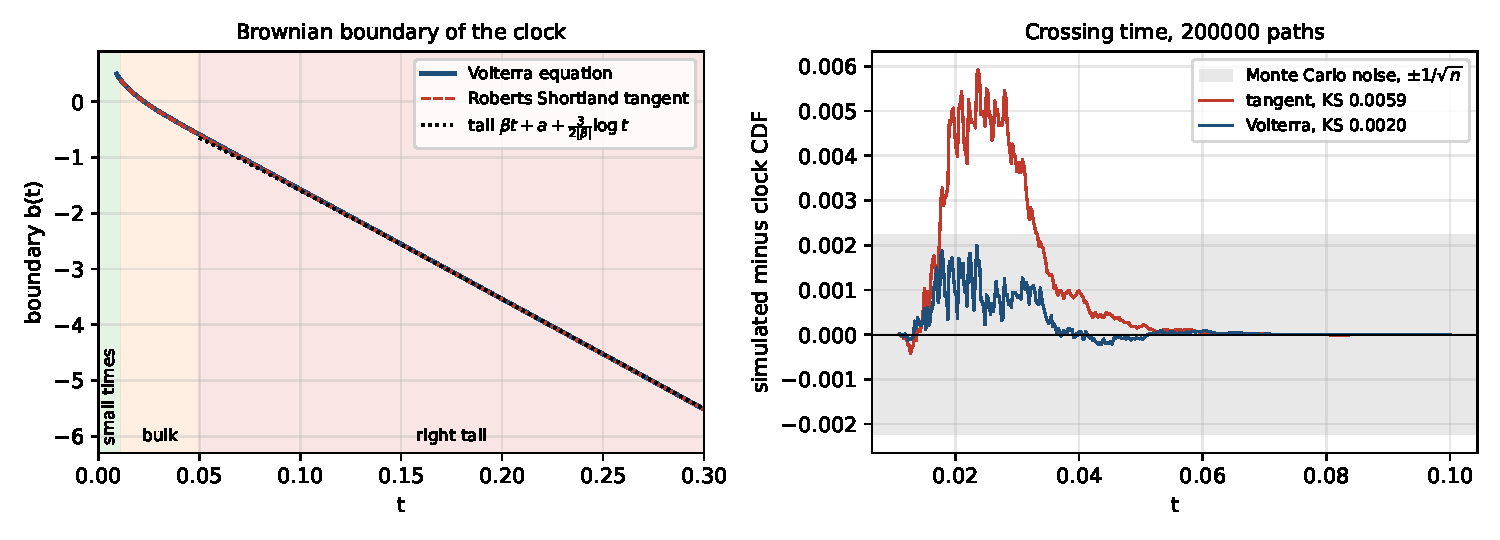
\includegraphics[width=\textwidth]{fig/threezones.pdf}
\caption{Left: the Brownian boundary of the clock computed from the Volterra equation, the Roberts Shortland tangent boundary, and the right tail asymptote with its logarithmic correction, over the three zones. Right: the simulated distribution function of the crossing time minus that of the clock, for both boundaries; the grey band is $\pm1/\sqrt n$, twice the largest standard error of a simulated distribution function.}
\label{fig:ch19:zones}
\end{figure}

\subsection{Williams' Gamma(2) structure: the tilt, a benchmark and its limits}\label{sec:ch19:williams}

Williams \cite{Williams90} and Biane, Pitman and Yor \cite{BPY01} showed that the variable $S_2=\sum_{n\ge1}\frac2{\pi^2n^2}\Gamma_n$ of Section~\ref{sec:ch18:reach} is a sum of two independent hitting times of level one by the three dimensional Bessel process started at $0$, and that $2\xi(s)=\E[(\pi S_2/2)^{s/2}]$, so that the P\'olya variable is $Y=\frac12\log(\pi S_2/2)$ tilted by $e^{Y/2}=(\pi S_2/2)^{1/4}$ (Section~\ref{ch:clock}; \cite[Section 16.2.1]{P26}). The Thorin measure of $S_2$ has atoms of mass two at the points $\pi^2n^2/2$, the Gamma(2) shape of a sum of two copies.

First, the tilt. Write $y$ for the variable of the P\'olya kernel, so that the value $y$ of $Y$ corresponds to the value $e^{2y}$ of $\pi S_2/2$. Moving the line of integration from the real axis to the line $\im y=\eta$, as in Proposition~\ref{prop:tilt}, rotates $e^{2y}$ by the angle $2\eta$ into the complex plane. The density of $S_2$, a theta series in its argument, continues analytically to the right half plane, and the boundary of that half plane, the natural boundary of the theta function \cite[Chapter 11, Section 1.4, and Chapter 5, Section 3.2]{Remmert98}, is reached exactly at $\eta=\pi/4$. So the admissible tilts of Proposition~\ref{prop:tilt} are the rotations of Williams' variable within the half plane of analyticity of its density, and the saving $e^{-\eta\theta}$ is the factor gained by that rotation.

Second, a benchmark. Since $\pi^2S_2/2=\sum_n\Gamma_n/n^2$, the Thorin measure of $\pi^2S_2/2$ is $2\sum_n\delta_{n^2}$, and in the square root variable its Cauchy flow $P_\varepsilon*2\sum_n\delta_n$ is explicit \cite[Section 16.4]{P26}. On this measure the distances of Section~\ref{ch:distances} separate the effects of the method from those of the arithmetic, and they need no separate computation: $\pi^2S_2/2$ is the sum of two independent copies of the sinh clock of Section~\ref{sec:ch3:bench}, so its distances follow from the closed forms of that section (Section~\ref{sec:open:calib}).

Third, the limits. Williams' atoms are the Dirichlet eigenvalues $\pi^2n^2/2$ of an interval, and they live on the Laplace side of the kernel. The zeros of $\xi$ live on the Mellin side of the same variable, and they reappear as unit atoms only on the Laplace side of the reciprocal. The Gamma(2) structure therefore gives positivity and an exact sampler \cite{Devroye86} on the kernel side, but it transfers no positivity to the Thorin measure of the clock. In particular it does not give a positive Gamma(2) scale mixture representation of the P\'olya density, a route that \cite[Section 12.6]{P26} excludes.
